\subsection*{\bfseries }
\clearpage
\textbf{1−4 インターネットのつながりについて知ろう}

教室内では無線通信を利用してインターネットを使用しています。第1回目の授業の最初に\ruby{皆}{みな}さんはインターネット\ruby{接続}{せつぞく}をしました。\ruby{実際}{じっさい}にはどこにつながっているかというと下の図のルータです。

\centering
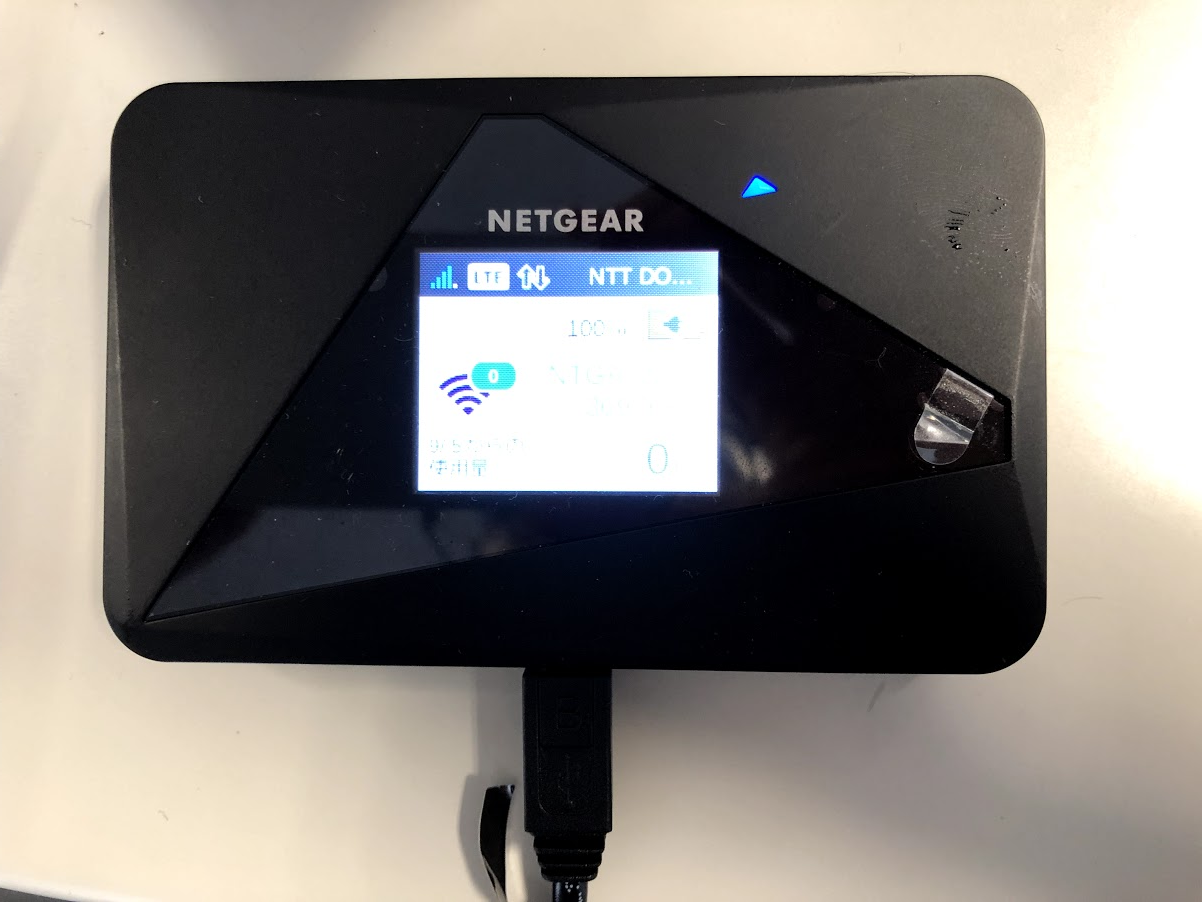
\includegraphics[width=8.186cm]{ome7-img011.png}
\flushleft


\bigskip


\bigskip


\bigskip


\bigskip


\bigskip


\bigskip


\bigskip

この機械のおかげで、みんなは教室内でインターネットをすることができているんだ。

どういう原理で、みんなのラズベリーパイでインターネットを使用できているか説明していくよ。

みんなのラズベリーパイは直接インターネットにつながってはいません。一度、ルータを経由しています。このルータのおかげで\ruby{複数}{ふくすう}のラズベリーパイやPCを同時にインターネットにアクセスさせることができるんだ。以下の図がイメージ図だよ。


\bigskip



\centering
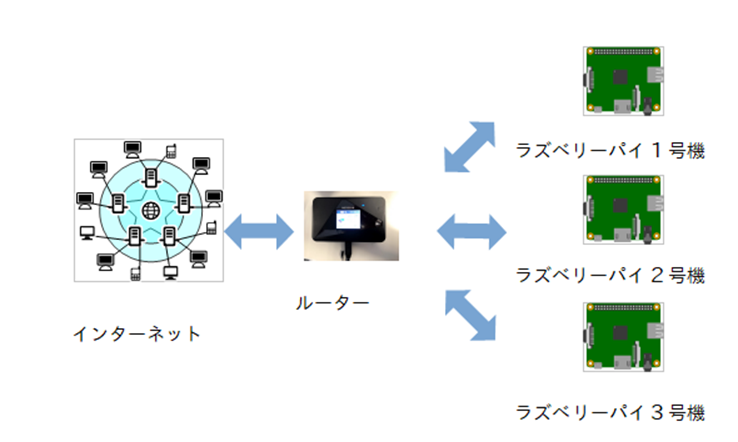
\includegraphics[width=\textwidth]{ome7-img012.png}
\flushleft


\bigskip

ではどのようにして複数台のラズベリーパイをインターネットに接続しているのでしょうか。それはルータに\textbf{グローバルIPアドレス}というものを\ruby{割}{わ}り当てて、ルータが他のラズベリーパイの代表として通信を行っています。どういうことかわかりずらいので、図でみていきましょう。



\centering
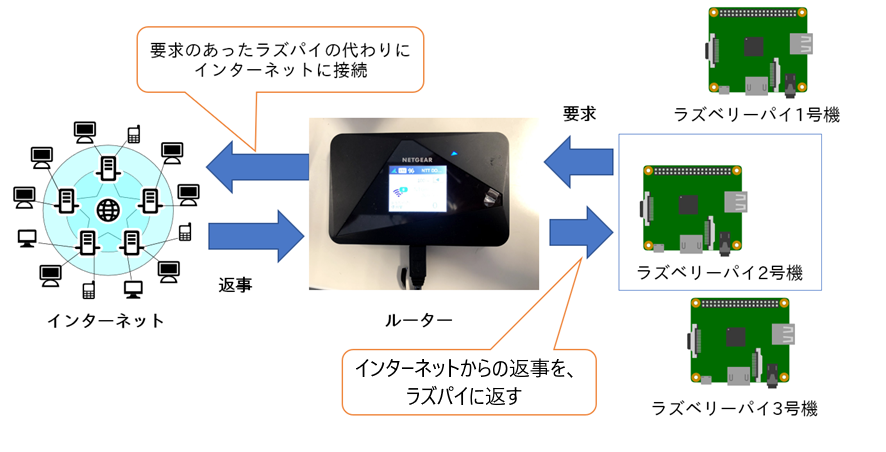
\includegraphics[width=0.9\textwidth]{ome7-img013.png}
\flushleft


\bigskip

図ではラズベリーパイ2号機がインターネットにアクセスし、何かしらの webサイトを観たいと要求したとします。その要求はまずルータのところにいき、ラズベリーパイ2号機の代わりにインターネットに接続します。その接続で、ルータはインターネット先から返事をもらい、そのインターネットからの返事をラズパイに返しています。

\centering
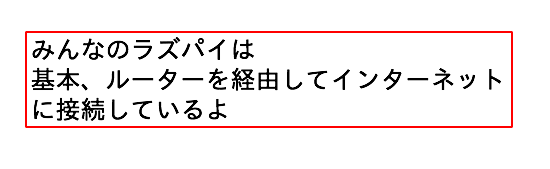
\includegraphics[width=0.9\textwidth]{ome7-img014.png}
\flushleft


\bigskip

\clearpage
これだけではうまくいかないことがあります。下の図をみてください。



\centering
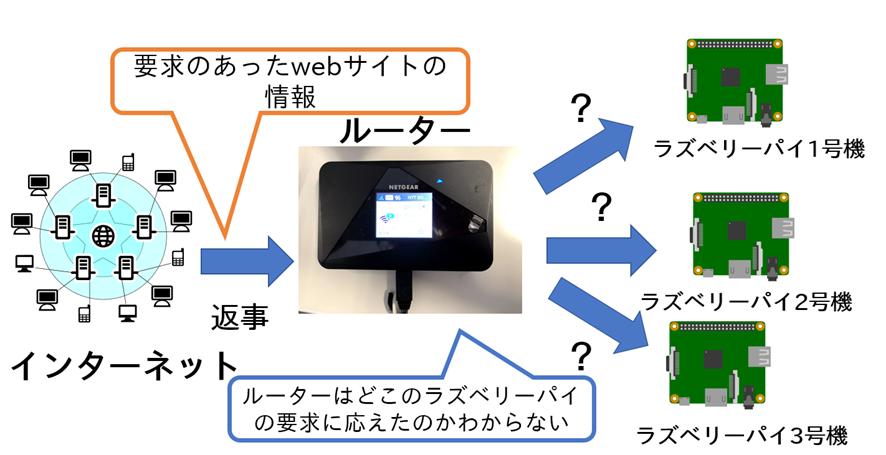
\includegraphics[width=0.9\textwidth]{ome7-img015.png}
\flushleft

どれかしらのラズベリーパイからwebサイトへの要求があり、ルータを経由してインターネットに接続します。そのあと、インターネットから要求のあったwebサイトの情報がルータにいきます。ここで問題が発生します。それはいったいのどのラズベリーパイの要求であったのかルータがわからないのです。\ruby{僕}{ぼく}らが、勝手にラズベリーパイ1号機、ラズベリーパイ2号機、ラズベリーパイ3号機と名前をつけて\ruby{判断}{はんだん}していても、そのことはルータはわかりません。そこでIPアドレスというものを使います。

ルータは自分を\ruby{含}{ふく}め、ローカルIPアドレスを割り当てています。このローカルIPアドレスでラズベリーパイを見分けています。
%\textbf{例題7−2で自分のラズベリーパイが接続しているグローバルIPアドレスを確認してみよう}

%\bigskip

\centering
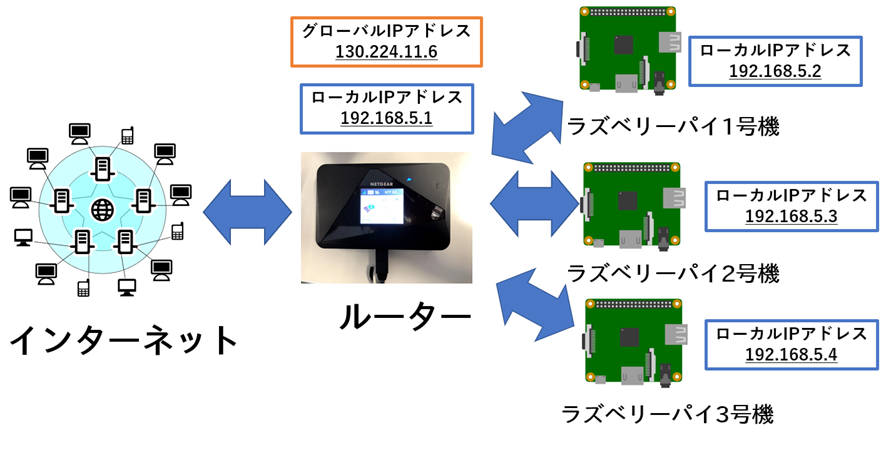
\includegraphics[width=0.9\textwidth]{ome7-img016.png}
\flushleft


\refstepcounter{Question}\theQuestion ルータはラズベリーパイたちを見分けるために何を割り当てていますか。\label{Q:globalIP}

\addBlank{答え}

\refstepcounter{Exercise}
\clearpage\subsection*{\theExercise ポケットWi-FiルータのグローバルIPアドレスを調べよう\label{E:router}}
\begin{minipage}[b]{0.58\textwidth}
	ターミナルを開き、”curl

	inet-ip.info”とコマンドを入力して、自分のラズベリーパイが接続しているWi-FiルータのグローバルIPアドレスを確認しよう

	curlコマンドはインターネットから情報を取ってくるときに使用します。今回は”inet-ip.info”というサイトからグローバルIPアドレスを調べてターミナルに\ruby{表示}{ひょうじ}させています。webブラウザから”inet-ip.info”にアクセスしてみると右の図のような形でグローバルIPアドレスを確認することもできます。

\end{minipage}
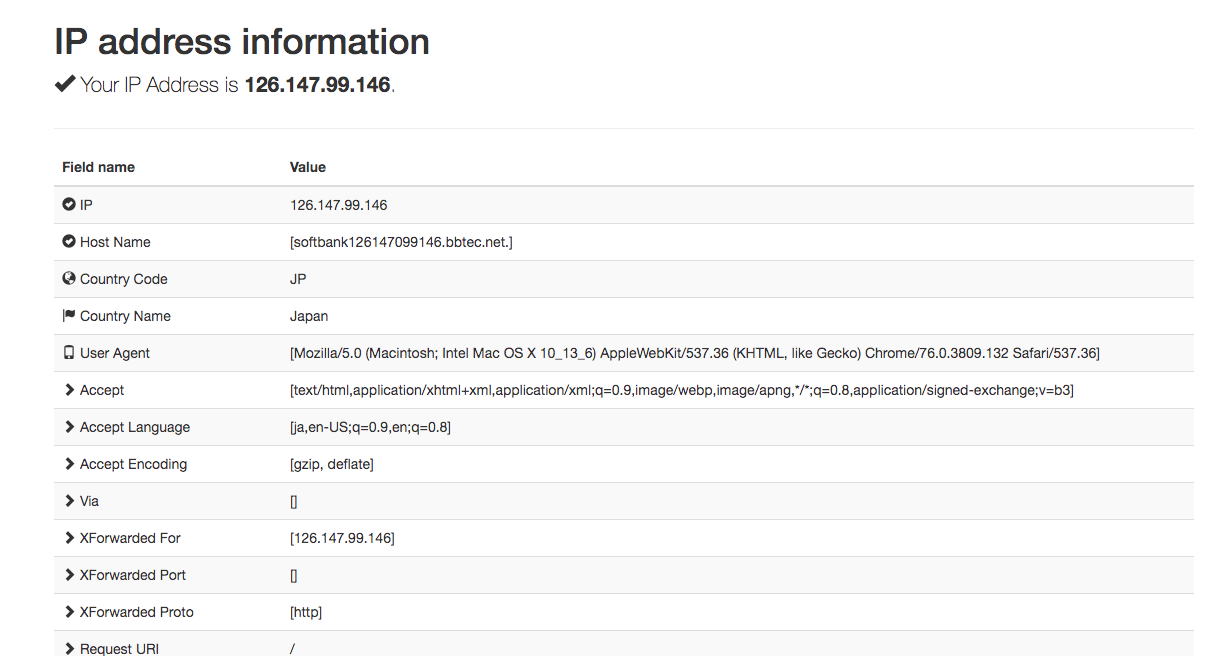
\includegraphics[width=0.4\textwidth]{ome7-img017.png}



\bigskip

{\bfseries
	方法}



\centering
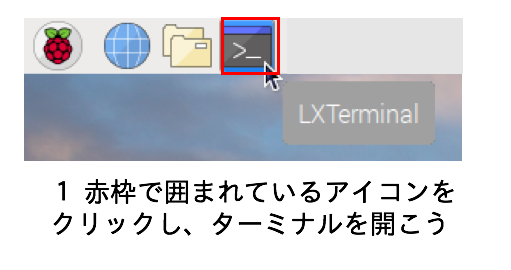
\includegraphics[width=0.85\textwidth]{ome7-img007.png}

\centering
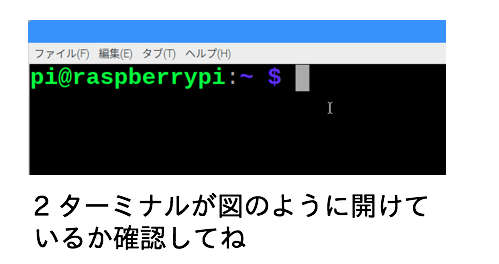
\includegraphics[width=0.85\textwidth]{ome7-img008.png}
\flushleft


\bigskip


\bigskip


\bigskip


\bigskip



\centering
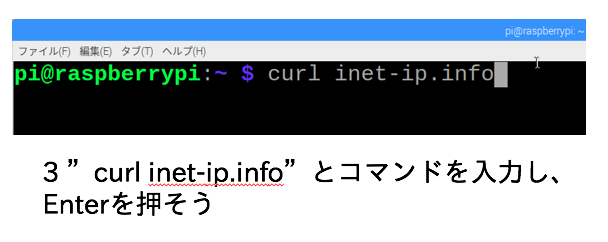
\includegraphics[width=0.85\textwidth]{ome7-img018.png}

\centering
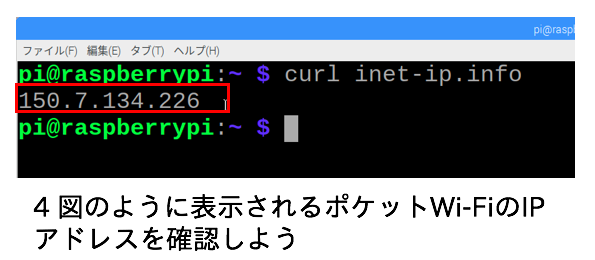
\includegraphics[width=0.85\textwidth]{ome7-img019.png}
\flushleft


\bigskip


\bigskip

{\bfseries
	調べたグローバルIPアドレスを書こう}


\bigskip


\centering
\begin{tabular}{|p{0.8\textwidth}|} \hline
	\\
	\\
	\\
	\\ \hline
\end{tabular}


\flushleft




\bigskip


\bigskip

{\bfseries
	グループの友達がしらべたポケットWi-FiのIPアドレスも教えてもらって書こう}



\bigskip


\centering
\begin{tabular}{|p{0.8\textwidth}|} \hline
	\\
	\\
	\\
	\\ \hline
\end{tabular}


\flushleft



\bigskip


\bigskip

